\subsection{Common Changes of Variables: Polar, Cylindrical, Spherical.}

There are a few very common transformations, and their Jacobians are worth paying special note to. One is the polar transformation for double integrals that we just saw.

\begin{claim}{Polar Jacobian}
Let $f(x,y)$ be a function over the region $R$, subject to the transformation
\begin{align*}
x(r,\theta)=&r\cos\theta\\
y(r,\theta)=&r\sin\theta.
\end{align*}
Then $\det(J)=r$ so $$\iint_R f(x,y)\ dA=\iint_S f_t(r,\theta)\cdot r\ d\ca{A}.$$
\end{claim}

\begin{exercise}{Polar Integration}
Let $D$ be the region between the circles of radius 2 and radius 5 centered at the origin that lies in the first quadrant. Evaluate $$\iint_D 2xy\ dA. $$
\end{exercise}

\begin{exercise}{Calculus II Formula for Polar Area}
Note that in general, for a given region $R$, $$\iint_R 1\ dA $$ computes the area of that region. Recall from Calculus II that $$\int_{\alpha}^{\beta}\frac{\big(r(\theta)\big)^2}{2}\ d\theta $$ gives the area between $r(\theta)$ and the origin between the angles $\alpha$ and $\beta$. 

\vspace{1em}

Let $R$ be the region where $0\leq r\leq r(\theta)$ and $\alpha \leq \theta\leq \beta$. Show that by converting to polar coordinates and evaluating the inner integral, $$\iint_R 1\ dA$$ gives the Calculus II formula for polar area.
\end{exercise}

\begin{exercise}{A White Whale}
An integral of considerable importance is $$\int_{-\infty}^{\infty}e^{-x^2}\ dx.$$ The function $e^{-x^2} $ is the basis of the normal distribution\footnote{Actually statistics uses $e^{-\frac{1}{2}x^2} $ rather than $e^{-x^2}$ because the extra constant factor makes variance come out nicer, but the logic here still holds without the extra constant.}, a very important idea in statistics. 

\vspace{1em}
\begin{center}
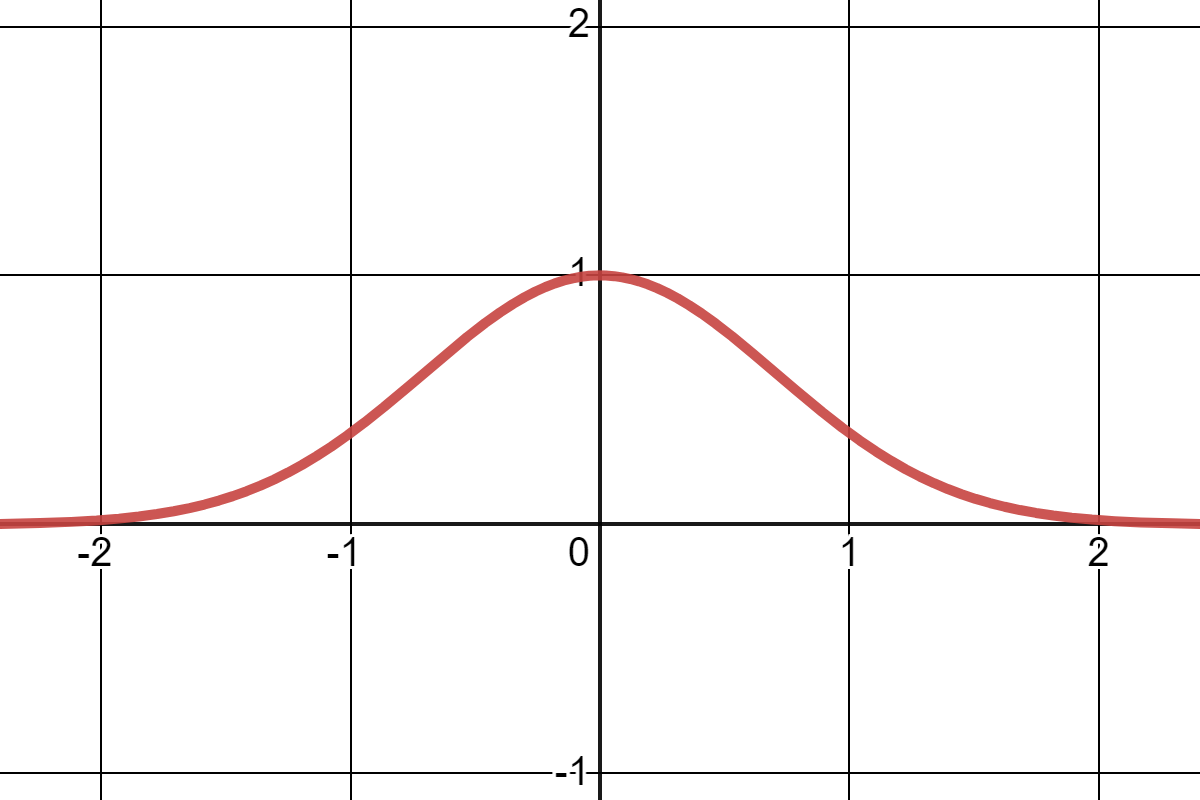
\includegraphics[scale=0.2]{Figures/531}\\ The graph of the function $e^{-x^2}$.
\end{center}
\vspace{1em}

In statistics, it is common practice to standardize distributions, so it is desired that we find some constant $c$ such that the area beneath $ce^{-x^2}$ is exactly 1. To do that, we need to be able to evaluate the integral above. There's just one problem-- which is that you can't find a closed form antiderivative for $e^{-x^2}$. 

\vspace{1em}

So what can we do? Let's let $$C=\int_{-\infty}^{\infty}e^{-x^2}\ dx.$$ Then let's consider instead a $3$-dimensional version of this integral, $$\iint_R e^{-x^2-y^2}\ dA $$ where $R=[-\infty,\infty]\times[-\infty,\infty].$ 

\vspace{1em}
\begin{center}
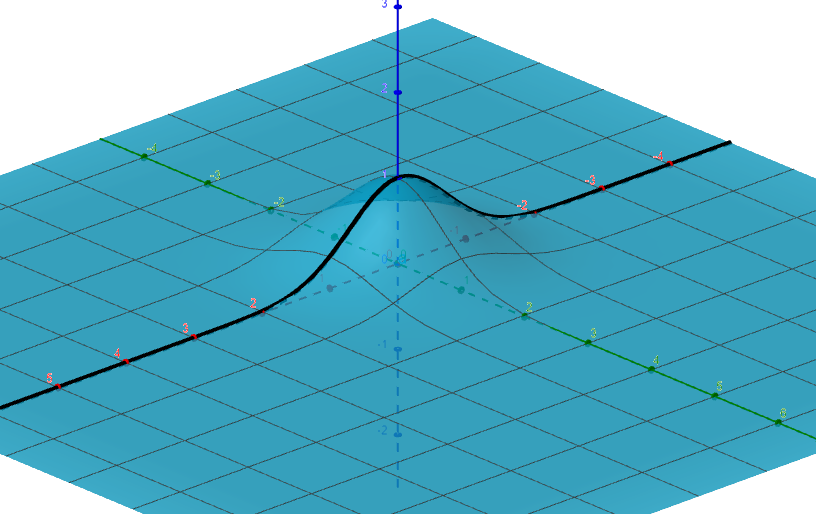
\includegraphics[scale=0.5]{Figures/532}\\ Click this \href{https://www.geogebra.org/3d/yrkngady}{geogebra link} for an interactive version of this graph.
\end{center}
\vspace{1em}
Consider the cross sectional area beneath the black curve in the graph above. The black curve is the portion of the surface that intersects the plane $y=0$. The area beneath that curve should be exactly $C$, or the value of the integral $$\int_{-\infty}^{\infty}e^{-x^2}\ dx.$$
If we move the line a little (which you can do in the interactive graph by using the slider), then you might notice that the new curve is the same curve as before, just scaled by some factor in the vertical direction. That is, the curve formed from the intersection of $y=c$ and $e^{-x^2-y^2}$ is a constant multiple of $e^{-x^2}$, and so it's area is some multiple of the unknown $C$ that we're looking for. In fact, the area of each cross section is just $C\cdot e^{-y^2}.$ We can reach back to Calculus II and compute the volume of this object using cross sectional areas as $$V=\int_{-\infty}^{\infty}C\cdot e^{-y^2}\ dy. $$ Since $C$ is a constant, we can factor it out of the integral as $$V=C\int_{-\infty}^{\infty}e^{-y^2}\ dy .$$ But remember that $$C=\int_{-\infty}^{\infty}e^{-x^2}\ dx=\int_{-\infty}^{\infty}e^{-y^2}\ dy.$$ So the volume beneath this surface is just $V=C^2$. \footnote{If you're having a hard time with the argument that $$\iint_R e^{-x^2-y^2}\ dA=\left(\int_{-\infty}^{\infty}e^{-x^2}\ dx\right)^2, $$ there is an excellent \href{https://youtu.be/cy8r7WSuT1I?t=551}{video from 3blue1brown} on the topic. He approaches the integral that we want to solve in a slightly more roundabout way that is accessible without double integration, but the visuals are excellent. The argument in question begins at about 9:11 in the video.}

\vspace{1em}

Great. So now we know that $$C^2=\iint_R e^{-x^2-y^2}\ dA $$ where $R=[-\infty,\infty]\times[-\infty,\infty].$ Now all that remains is to calculate that integral. Use a polar transformation to compute the integral and then give the value of $C$.

\end{exercise}

\hypertarget{cylind}{Another common transformation is the triple integral in cylindrical coordinates.}

\begin{exercise}{Cylindrical Jacobian}
Cylindrical coordinates in 3-space are much like polar coordinates in 2-space. To convert to cylindrical coordinates, you'll use the transformation:
\begin{align*}
x(r,\theta,z)=&r\cos\theta\\
y(r,\theta,z)=&r\sin\theta\\
z(r,\theta,z)=&z.
\end{align*}
Find the Jacobian and show that $|\det(J)|=r$ for this transformation.
\end{exercise}

\begin{exercise}{Cylindrical Integration}
Let $D$ be the region that lies below the plane $z=x+2$ and above the $xy$-plane and between the cylinders $x^2+y^2=1$ and $x^2+y^2=4$. Use a change to cylindrical coordinates to evaluate $$\iiint_D y\ dV. $$
\end{exercise}

\hypertarget{spherical}{A third common transformation is the triple integral in spherical coordinates}. Spherical coordinates have a few different methods of computing-- here we use the typical mathematical convention where $\theta$ refers to the \textit{azimuthal angle} and $\phi$ refers to the \textit{polar angle}. That is, $\theta$ is the angle in standard position in the $xy$-plane, and $\phi$ is the angle from the positive $z$-axis to the point. Either way, we use $\rho$ to denote the spherical radius (i.e. the distance from the point to the origin). That is, $\rho,$ $ \theta$ and $\phi$ are as below:

\begin{center}%UPDATE DIAGRAM
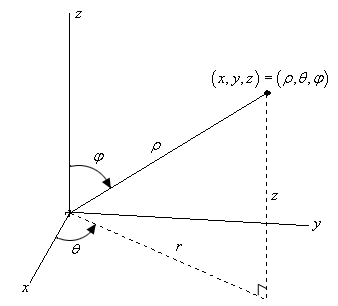
\includegraphics[scale=0.5]{Figures/sphericalcoord}
\end{center}

Note that many sources (usually physics sources) switch $\theta$ and $\phi$. For example, if you go to the \href{}{Wikipedia page on the Spherical coordinate system}, you can see that they use the convention that $\theta$ is the polar angle and $\phi$ is the azimuthal angle. They also use $r$ for the spherical radius. While the physics convention has an ISO standard on its side, I argue that it is more correct to use a consistent $\theta$ between polar, cylindrical and spherical coordinates, and similarly think that we should not use $r$ for the spherical radius as it differs from the polar and cylindrical radius.

\begin{exercise}{Spherical Jacobian}
Spherical coordinates are another analogue to polar coordinates in 2-space, but utilize a radius and two angles. To convert to spherical coordinates, you'll use the transformation:
\begin{align*}
x(\rho,\phi,\theta)=&\rho\sin\phi\cos\theta\\
y(\rho,\phi,\theta)=&\rho\sin\phi\sin\theta\\
z(\rho,\phi,\theta)=&\rho\cos\phi.
\end{align*}
Find the Jacobian and show $|\det(J)|=\rho^2\sin\phi$ for this transformation.
\end{exercise}

\begin{exercise}{Spherical Integration}
Let $D$ be the region between the upper half of the sphere $x^2+y^2+z^2=1$ and the $xy$-plane. Evaluate $$\iiint_D 16x\ dV. $$
\end{exercise}
